\chapter{Introducción}\label{ch:chapter_1}


\section{Antecedentes}

El desarrollo de este Trabajo de Fin de Grado (TFG) surge de una necesidad surgida en mi faceta profesional, donde la
tarea de leer y extraer información de documentos representa una carga significativa para la empresa en la que trabajo
en la actualidad.

Este problema no es exclusivo de mi actual empresa actual, sino que es una realidad común en una variedad de sectores
incluyendo entre otros:

\begin{itemize}
    \item Compañías de seguros
    \item Instituciones educativas
    \item Empresas del sector sanitario
    \item Empresas de gestión de recursos humanos
    \item Entidades financieras
\end{itemize}

Estas empresas y organizaciones se enfrentan el reto constante de gestionar grandes volúmenes de documentación, lo cual
resalta la importancia y la necesidad de soluciones automatizadas que permitan extraer información de dichos documentos.

Además, durante la asignatura del Grado de Ingeniería Informática 47 Proyecto de Ingeniería del Software, tuve la
oportunidad de desarrollar una base técnica preliminar que he utilizado como la base para la realización de este TFG\@.


\section{Planteamiento del problema}

Las tipologías de empresas que hemos visto en el apartado anterior se enfrentan a la necesidad de procesar una enorme
cantidad de documentos.

Por ejemplo una empresa que gestiona seguros de coche, deberá recibir un paquete de datos de cada nuevo cliente que
contendrá entre otros los siguientes documentos:

\begin{itemize}
    \item Documentos de identidad del titular y los tomadores
    \item Permiso de conducción de los tomadores
    \item Ficha técnica y permiso de circulación del vehículo
    \item Recibo del impuesto de vehículo de tracción mecánica
\end{itemize}

La forma tradicional de obtener la información que contienen dichos documentos consiste en que un operario reciba los
documentos, los abra y los introduzca en el sistema.
Esta metodología tradicional enfrenta una problemática significativa:

\begin{itemize}
    \item \textbf{Elevado coste}
    El personal dedicado a estas tareas genera un gasto que impacta directamente en el coste operativo de la
    organización.
    \item \textbf{Demora en los tiempos de tramitación}
    La tramitación manual implica que los documentos no van a ser procesados en el momento en que son recibidos, sino
    que deberán esperar a que un operario esté disponible para ocuparse de esta tarea.
    \item \textbf{Pobre asignación de recursos}
    Los recursos invertidos en la tramitación manual de documentos podrían ser asignados a actividades que aporten un
    mayor valor a la organización.
    Esto incluye tareas como la innovación, el desarrollo estratégico y el servicio al cliente, entre otros.
    \item \textbf{Errores manuales}
    La tramitación manual de documentos es intrínsecamente susceptible a los errores humanos.
\end{itemize}

Ante esta situación, se hace necesario el desarrollo de soluciones responsables de automatizar el proceso de extracción
de la información.


\section{Justificación}

La relevancia de este TFG se fundamenta en la necesidad de implementar soluciones que automatizar el proceso de
extracción de la información contenida en documentos.

\begin{itemize}
    \item
    Desde el punto de vista profesional este proyecto responde a una necesidad real de desarrollar una solución
    que permita la recuperación de la información contenida en documentos de diversa índole.
    \item
    Desde la perspectiva académica, el desarrollo de un sistema de extracción automática de información aborda
    competencias clave en la ingeniería informática, el diseño de sistemas, la programación, y las buenas prácticas de
    desarrollo de software.
\end{itemize}

En resumen, este TFG no solo es una oportunidad para aplicar habilidades y conocimientos técnicos adquiridos durante el
grado, sino también una contribución a la innovación que aplica directamente en mi ámbito profesional.


\section{Objetivos}

El propósito central de este trabajo es la creación de un sistema que permita la extracción automática de documentos.

\begin{figure}[ht]
    \begin{center}
        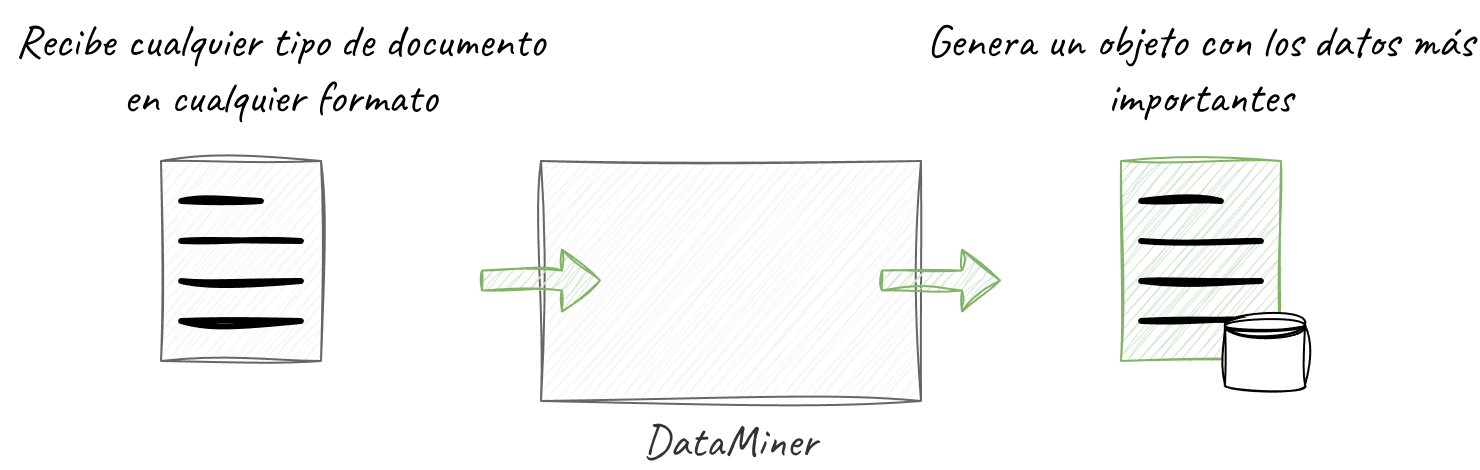
\includegraphics[width=\textwidth]{./chapter/1/images/chapter_1.overview}
        \caption{Visión general del funcionamiento del sistema}
        \label{fig:chapter_1.overview}
    \end{center}
\end{figure}

Tal y como se puede ver en la figura~\ref{fig:chapter_1.overview} el funcionamiento es el siguiente:

\begin{enumerate}
    \item El sistema recibe un documento de cualquier tipo en cualquier formato.
    \item
    Si el sistema puede procesar el documento, tanto por el formato, como por el tipo de documento, genera un objeto que
    contiene la información relevante del documento recibido.
\end{enumerate}

Como este objetivo puede resultar demasiado ambicioso, el alcance de este TFG quedará limitado a los siguientes
objetivos específicos que aparecen en la figura~\ref{fig:chapter_1.specific_a}.

\begin{enumerate}
    \item
    Desarrollar un sistema capaz de convertir documentos PDF en documentos de texto plano que puedan ser procesados.
    \item Implementar dos casos de uso dentro del sistema:
    \begin{enumerate}
        \item Procesar contratos de arrendamiento de vivienda entre particulares.
        \item Procesar contratos de compraventa de vehículo entre particulares.
    \end{enumerate}
\end{enumerate}

\begin{figure}[ht]
    \begin{center}
        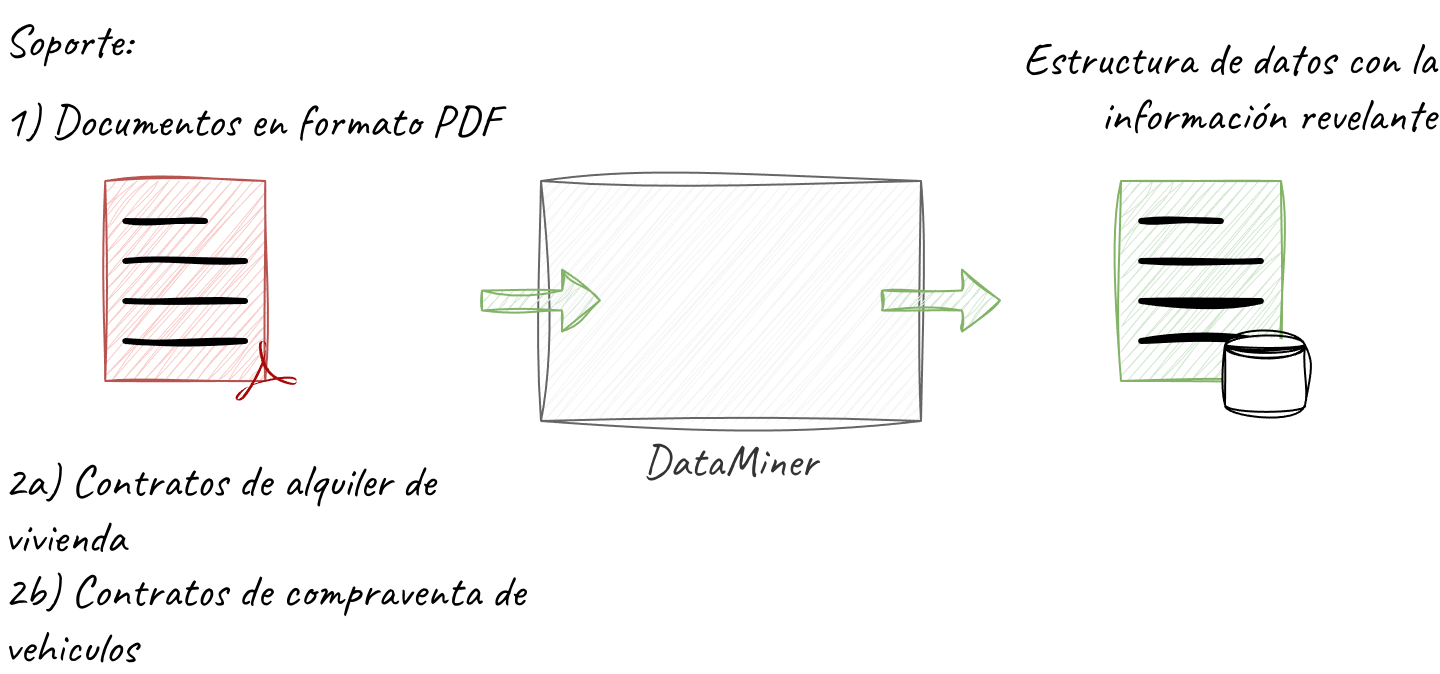
\includegraphics[width=\textwidth]{chapter/1/images/chapter_1.specific_a}
        \caption{Objetivos específicos del sistema}
        \label{fig:chapter_1.specific_a}
    \end{center}
\end{figure}

Además, tal como aparece en la figura~\ref{fig:chapter_1.specific_b} vamos a necesitar dos elementos adicionales para
completar este trabajo.

\begin{enumerate}
    \item Desarrollar un conjunto de pruebas, que permita realizar las pruebas oportunas durante el desarrollo del
    proyecto, y que en su conclusión nos permita evaluar como de preciso es el sistema.
    \item Desarrollar interfaces que permitan comunicarse con el sistema:
    \begin{enumerate}
        \item  Una interfaz web
        \item  Una interfaz de línea de comandos
    \end{enumerate}
\end{enumerate}

\begin{figure}[ht]
    \begin{center}
        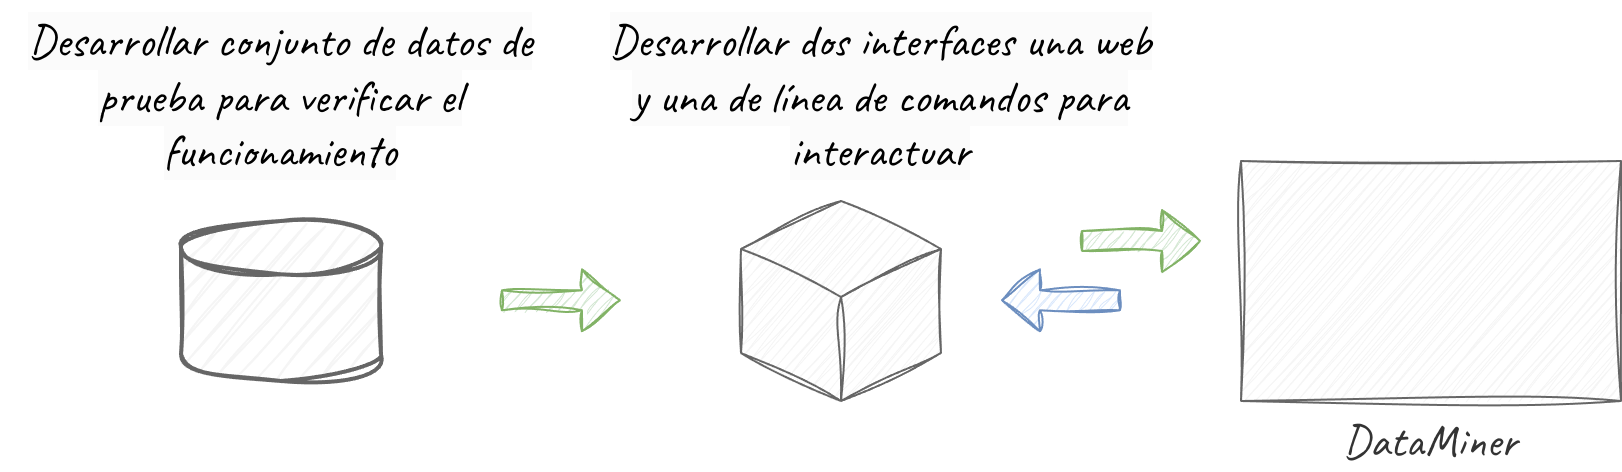
\includegraphics[width=\textwidth]{chapter/1/images/chapter_1.specific_b}
        \caption{Conjunto de datos prueba e interfaces interactuando con el sistema}
        \label{fig:chapter_1.specific_b}
    \end{center}
\end{figure}

Además, el sistema estará diseñado para introducir nuevas características de una forma sencilla.
Por ejemplo estas son algunas características que pueden ser añadidas fácilmente.

\begin{enumerate}
    \item
    Procesar nuevos tipos de documentos, como por ejemplo formatos de office como microsoft word o microsoft excel,
    o formatos de video o audio, etc.
    \item
    Procesar nuevos tipos de documentos, como por documentos de identidad, acuerdos de confidencialidad, documentos
    de impuestos, etc.
\end{enumerate}
